\section{简介}

%%%%%%%%%%%%%%%%%%%%%%%%%%%%%%%%%%%%%%%%%%%%%%%%%%%%%%%%%%%%%%%%%%%%%%%%%%%%%%%%%%%
\subsection{VCS}
%%%%%%%%%%%%%%%%%%%%%%%%%%%%%%%%%%%%%%%%%%%%%%%%%%%%%%%%%%%%%%%%%%%%%%%%%%%%%%%%%%%

\begin{frame}{第一代\en{VCS}}
    \begin{columns}[onlytextwidth]
        \column{.6\textwidth}
        \centering
        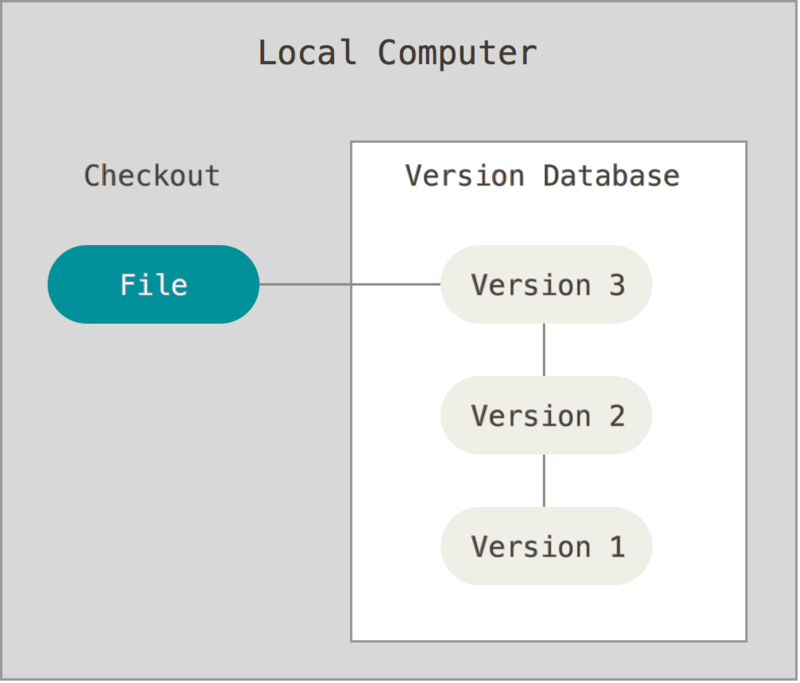
\includegraphics[scale=0.24]{figures/local.png}\\
        \column{.4\textwidth}
        \begin{itemize}
            \item 单点架构
            \item 本地存储
        \end{itemize}
    \end{columns}
\end{frame}

\begin{frame}{第二代\en{VCS}}
    \begin{columns}[onlytextwidth]
        \column{.6\textwidth}
        \centering
        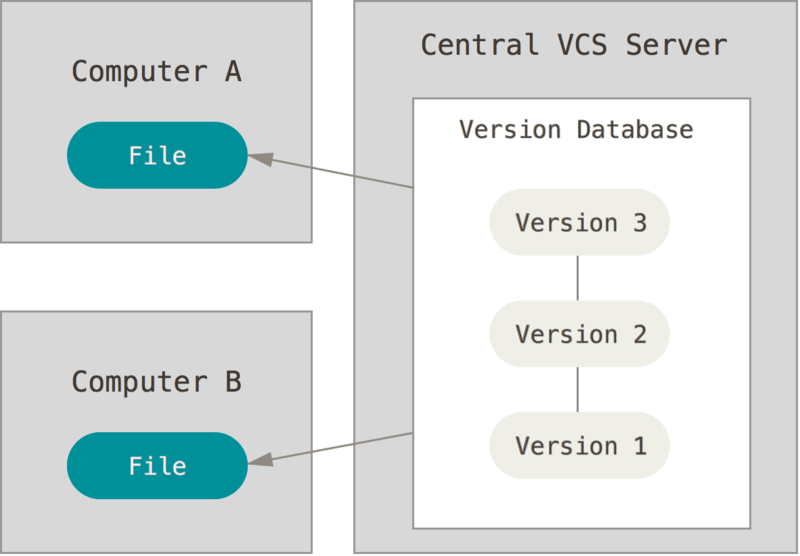
\includegraphics[scale=0.24]{figures/centralized.png}\\
        \column{.4\textwidth}
        \begin{itemize}
            \item \en{C/S}架构
            \item 中心化存储
            \item 典型代表:\en{CVS/Svn}
        \end{itemize}
    \end{columns}
\end{frame}

\begin{frame}{第三代\en{VCS}}
    \begin{columns}[onlytextwidth]
        \column{.6\textwidth}
        \centering
        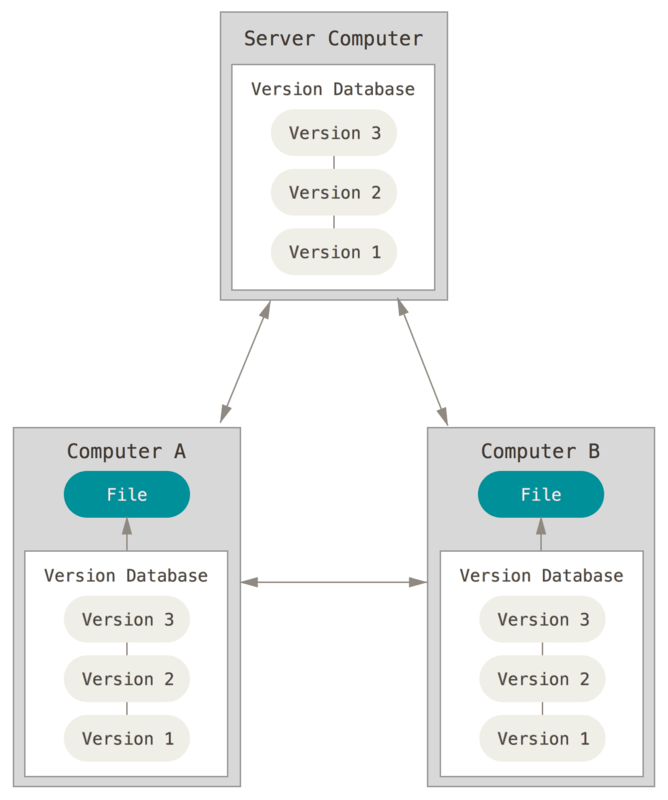
\includegraphics[scale=0.24]{figures/distributed.png}\\
        \column{.4\textwidth}
        \begin{itemize}
            \item \en{P2P}架构
            \item 分布式存储
            \item 典型代表:\en{Git}
        \end{itemize}
    \end{columns}
\end{frame}

%%%%%%%%%%%%%%%%%%%%%%%%%%%%%%%%%%%%%%%%%%%%%%%%%%%%%%%%%%%%%%%%%%%%%%%%%%%%%%%%%%%
\subsection{Git}
%%%%%%%%%%%%%%%%%%%%%%%%%%%%%%%%%%%%%%%%%%%%%%%%%%%%%%%%%%%%%%%%%%%%%%%%%%%%%%%%%%%

\begin{frame}
    \begin{columns}[onlytextwidth]
        \column{.5\textwidth}
        \centering
        
\includegraphics[scale=0.24]{figures/git.png}\\
        \column{.5\textwidth}
        \begin{itemize}
            \item 为自由之信仰而生
            \item 出身名门,天生不凡
            \item 实力碾压一切牛鬼蛇神
        \end{itemize}
    \end{columns}
\end{frame}

\begin{frame}[t]{\en{Git}之父}
    \begin{columns}[onlytextwidth]
        \column{.5\textwidth}
        \begin{exampleblock}{Linus Torvalds}
            \begin{itemize}
                \item \en{Linux}之父
                \item 世界级开源领袖
                \item 人类史上十大黑客之一
            \end{itemize}
        \end{exampleblock}
        \column{.5\textwidth}
        \centering
        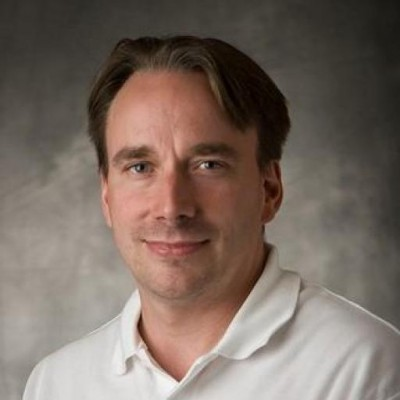
\includegraphics[height=28ex,width=24ex]{figures/linus.jpg}\\
    \end{columns}
\end{frame}

\begin{frame}{\en{Git}的目标}
    \begin{itemize}
        \item Speed
        \item Simple design
        \item Strong support for non-linear development (thousands of parallel branches)
        \item Fully distributed
        \item Able to handle large projects like the Linux kernel efficiently (speed and data size)
    \end{itemize}
\end{frame}

\begin{frame}{\en{Git}的优势}
    \begin{itemize}
        \item 业界最流行方案,主流\en{IDE}默认集成
        \item \href{https://git-scm.com/about/small-and-fast}{运行速度比\en{Svn}快数倍,甚至数百倍}
        \item 分布式架构,支持离线完成绝大多数工作
        \item 极其轻量的本地分支
        \item 便捷的分支合并流程
        \item 强大的数据安全保证
        \item 创新的缓存区设计
        \item 免费且开源
        \item $\cdots$
    \end{itemize}
\end{frame}

\begin{frame}{Git PK Svn}
    \centering
    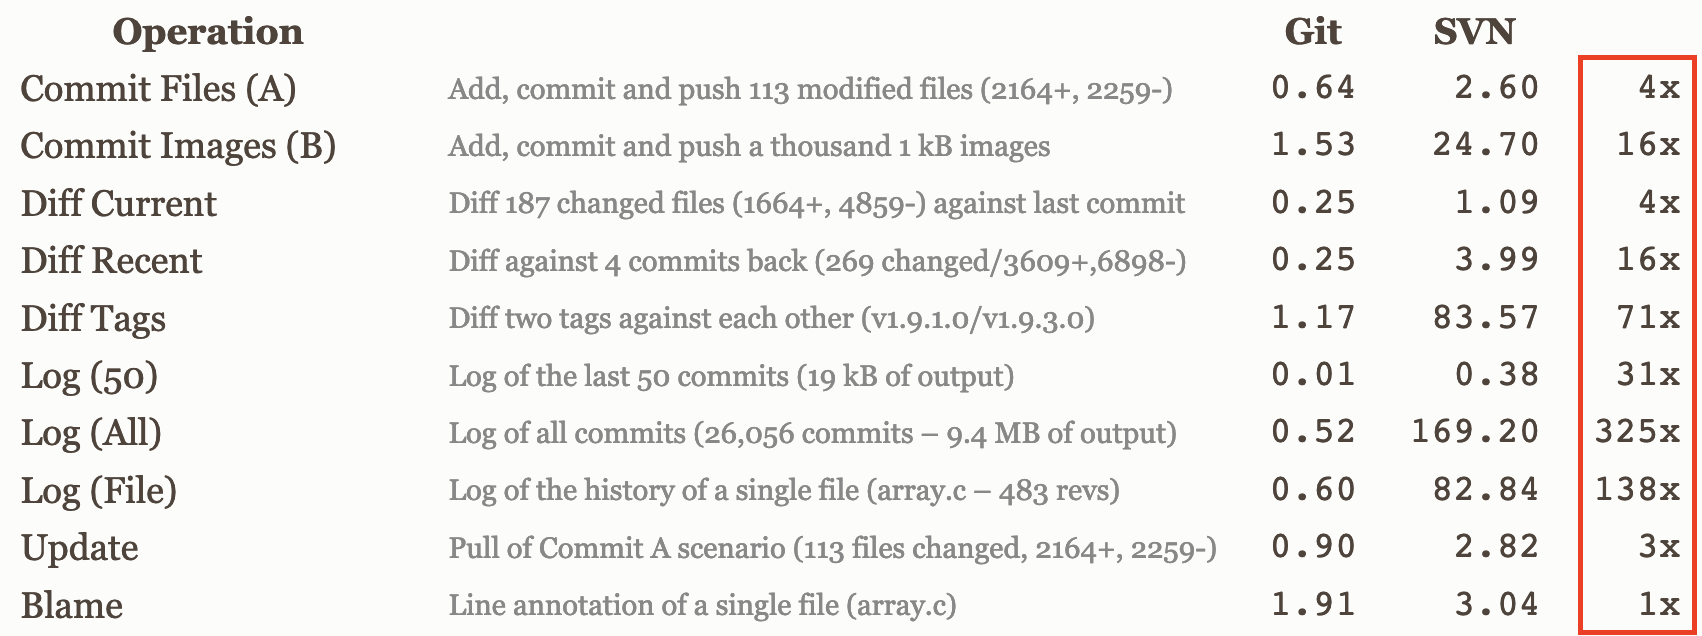
\includegraphics[scale=0.4]{figures/git_vs_svn.png}
\end{frame}

\begin{frame}{\en{Git}的应用场景}
    \begin{itemize}
        \item 版本控制(代码、文档等)
        \item 多人协作
        \item 项目管理(GitHub/GitLab)
        \item 兼容\en{Svn}
        \item CI/CD
        \item $\cdots$
    \end{itemize}
\end{frame}